\documentclass{beamer}
\usepackage{graphicx}
\usepackage{amsmath}

\title{Monetary and Fiscal Policy Analysis --- December 16, 2008}
\author{Anuj Patel, Charles Ancel, and Henry Szklanny (Team Two)}
\date{August 2nd, 2024}

\begin{document}

\frame{\titlepage}

\section{Introduction}
\begin{frame}
    \frametitle{Introduction}
    Good evening, everyone. My name is Charles Ancel, and today I will be presenting an analysis of the monetary and fiscal policy decisions around December 16, 2008. This presentation is part of, ECON 425, a course on Macroeconomic Policy at University of Illinois. Let's dive in.
\end{frame}

\section{Contextual Information}
\begin{frame}
    \frametitle{Contextual Information}
    \begin{itemize}
        \item The FOMC had recently lowered the federal funds rate by 50 basis points to 1\% in response to slowing economic activity.
        \item On December 1st, the National Bureau of Economic Research officially declared that the US had entered a recession.
        \item Key indicators showed significant declines in retail sales, manufacturing, real estate purchases, and business and consumer lending.
        \item Labor markets were weakening, price pressures were decreasing, and financial markets were experiencing further declines as pessimism grew.
        \item Projected a 5\% fall in GDP over the next two quarters, with unemployment rising to about 8\% in 2010 and PCE inflation remaining around 1\% for 2009 and 2010.
    \end{itemize}
\end{frame}

\section{Contextual Data}
\begin{frame}
    \frametitle{Contextual Data --- GDP}
    \begin{itemize}
        \item Examining the GDP from Q4 2003 to Q4 2013.
        \item The US economy was in a recession during this period.
        \item GDP at the end of Q4 2008 was approximately 14,608.209 billion USD.
    \end{itemize}

\end{frame}

\begin{frame}
    \frametitle{Graph --- GDP}
    \begin{figure}[h!]
        \centering
        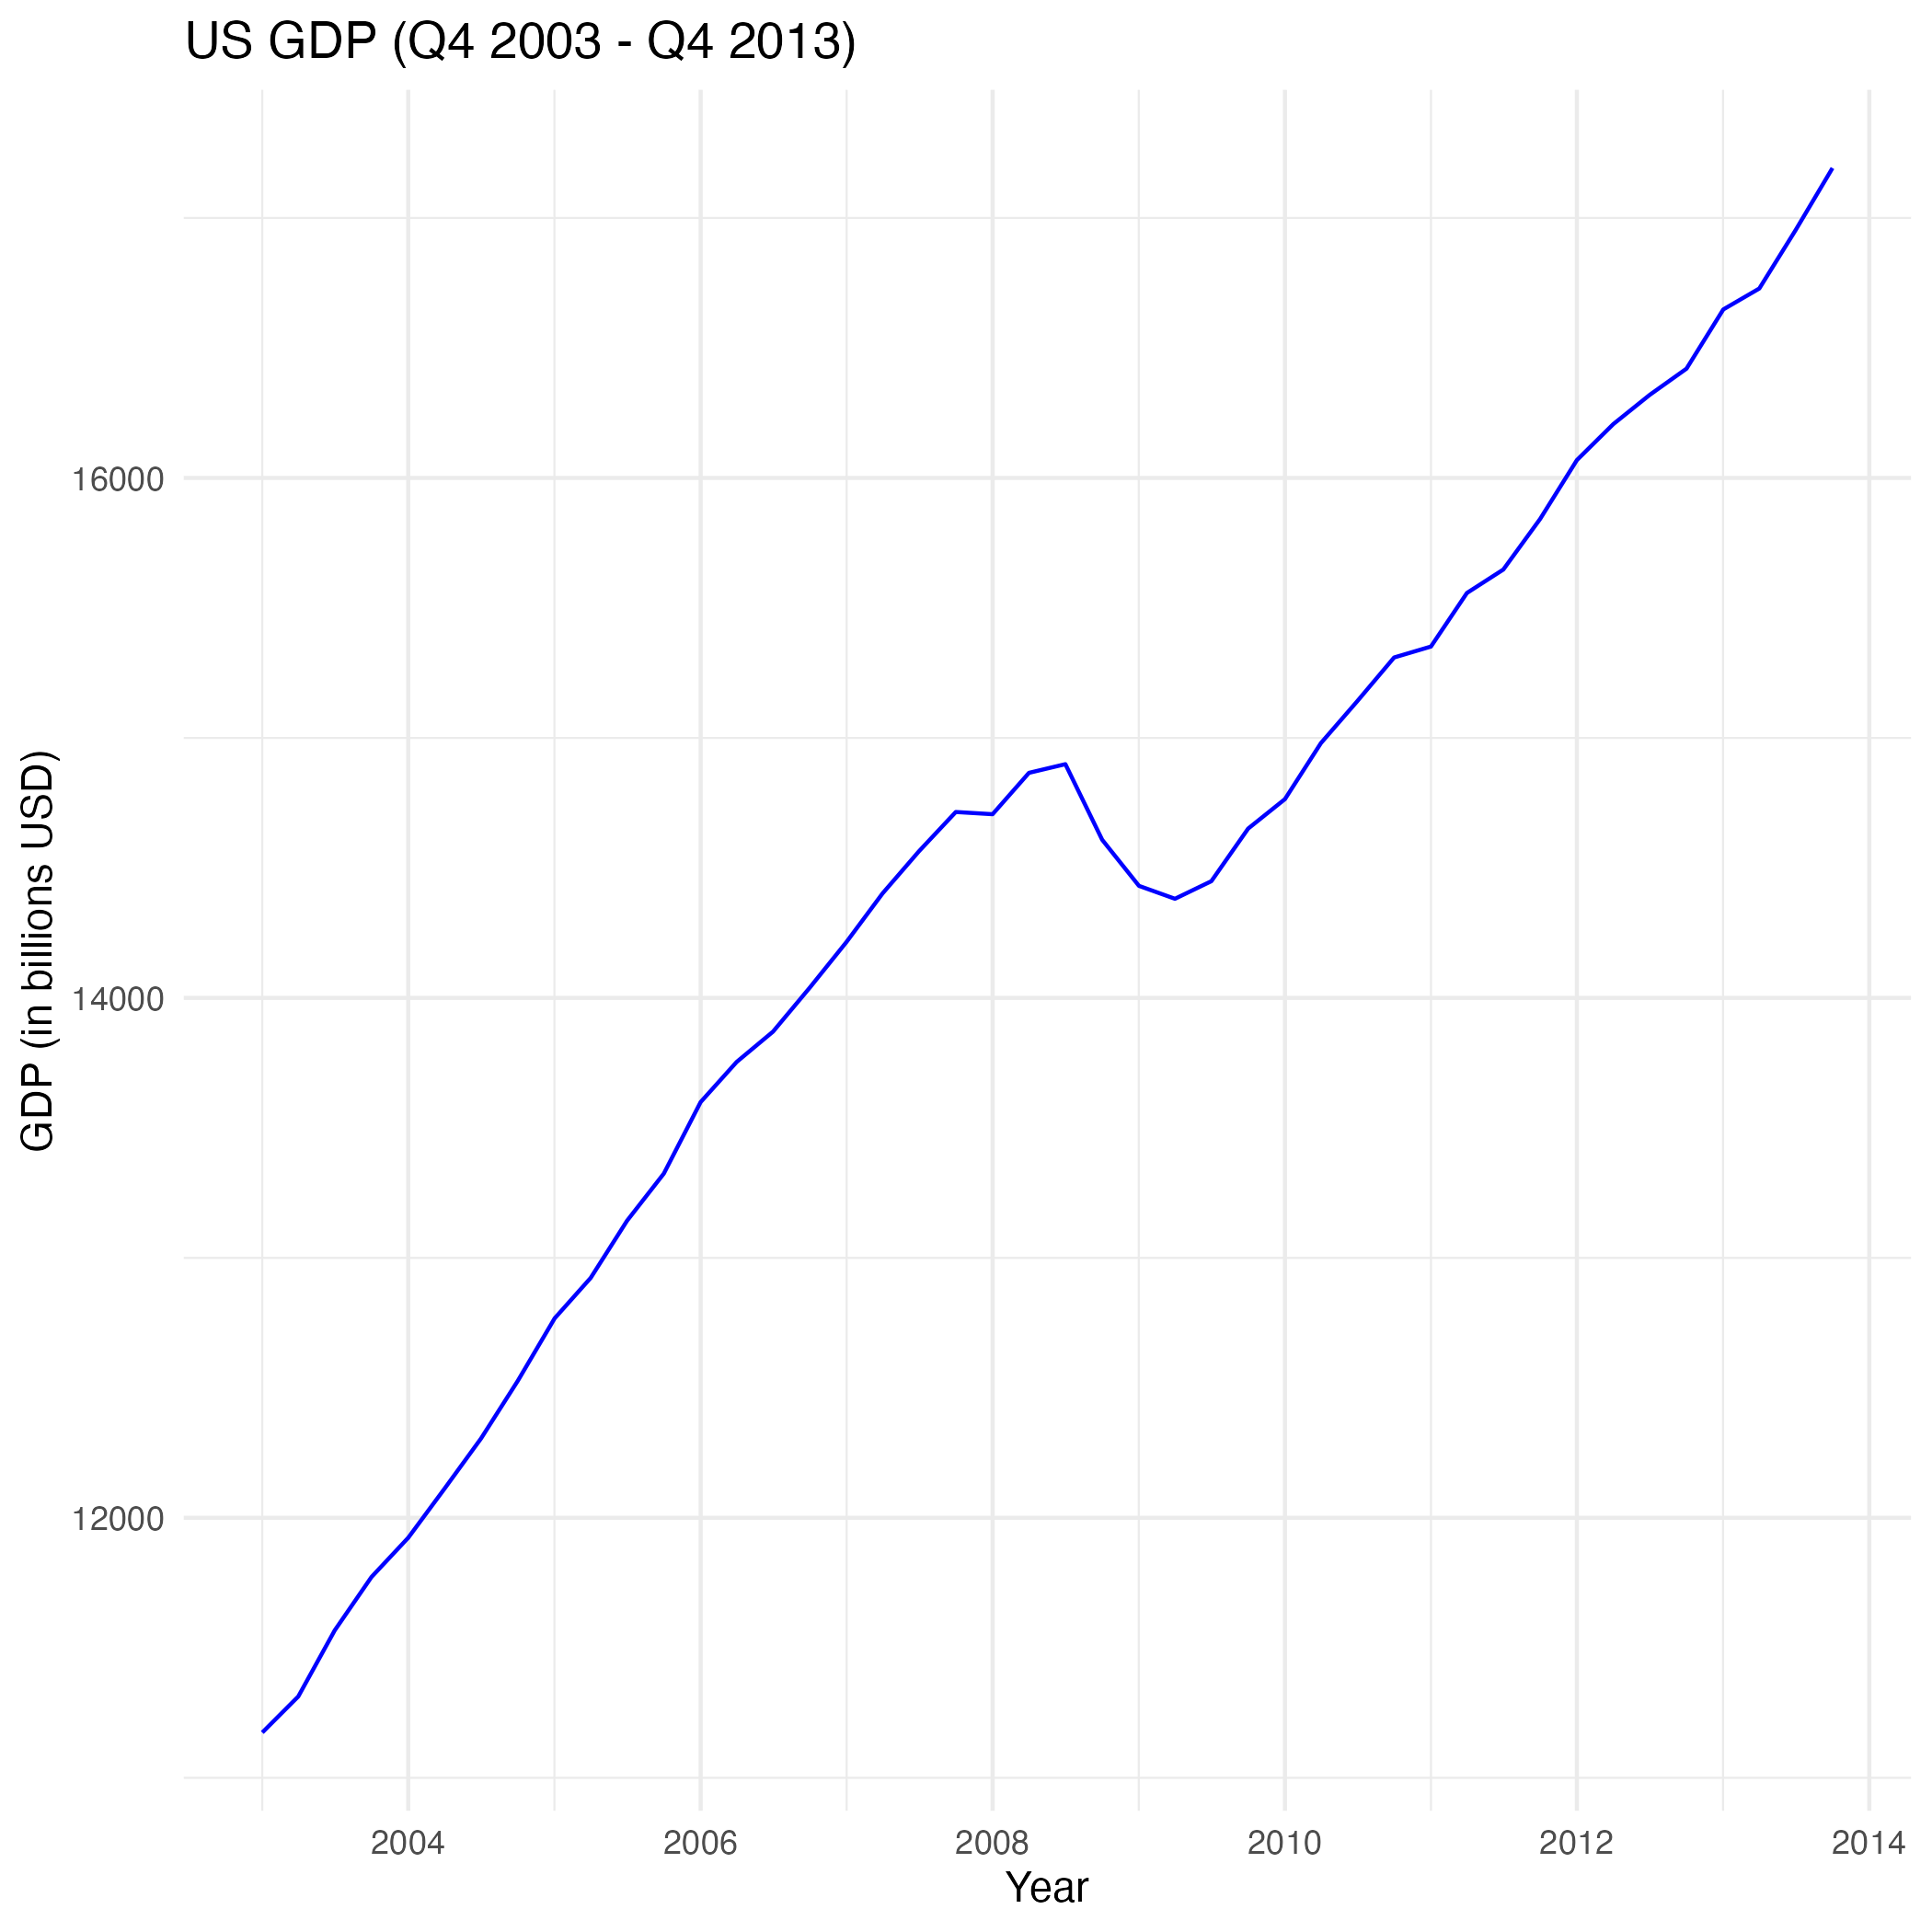
\includegraphics[width=0.8\textwidth]{/Users/cancel/Personal/Coursework/Econ425/FinalWork/R/gdp_graph.png}
    \end{figure}
\end{frame}

\begin{frame}
    \frametitle{Contextual Data --- Inflation}
    \begin{itemize}
        \item Inflation as measured by the Consumer Price Index (CPI).
        \item Annual percentage change in the cost of a basket of goods and services.
        \item Inflation dropped dramatically, becoming negative at some point in 2009.
    \end{itemize}
\end{frame}

\begin{frame}
    \frametitle{Graph --- Inflation}
    \begin{figure}[h!]
        \centering
        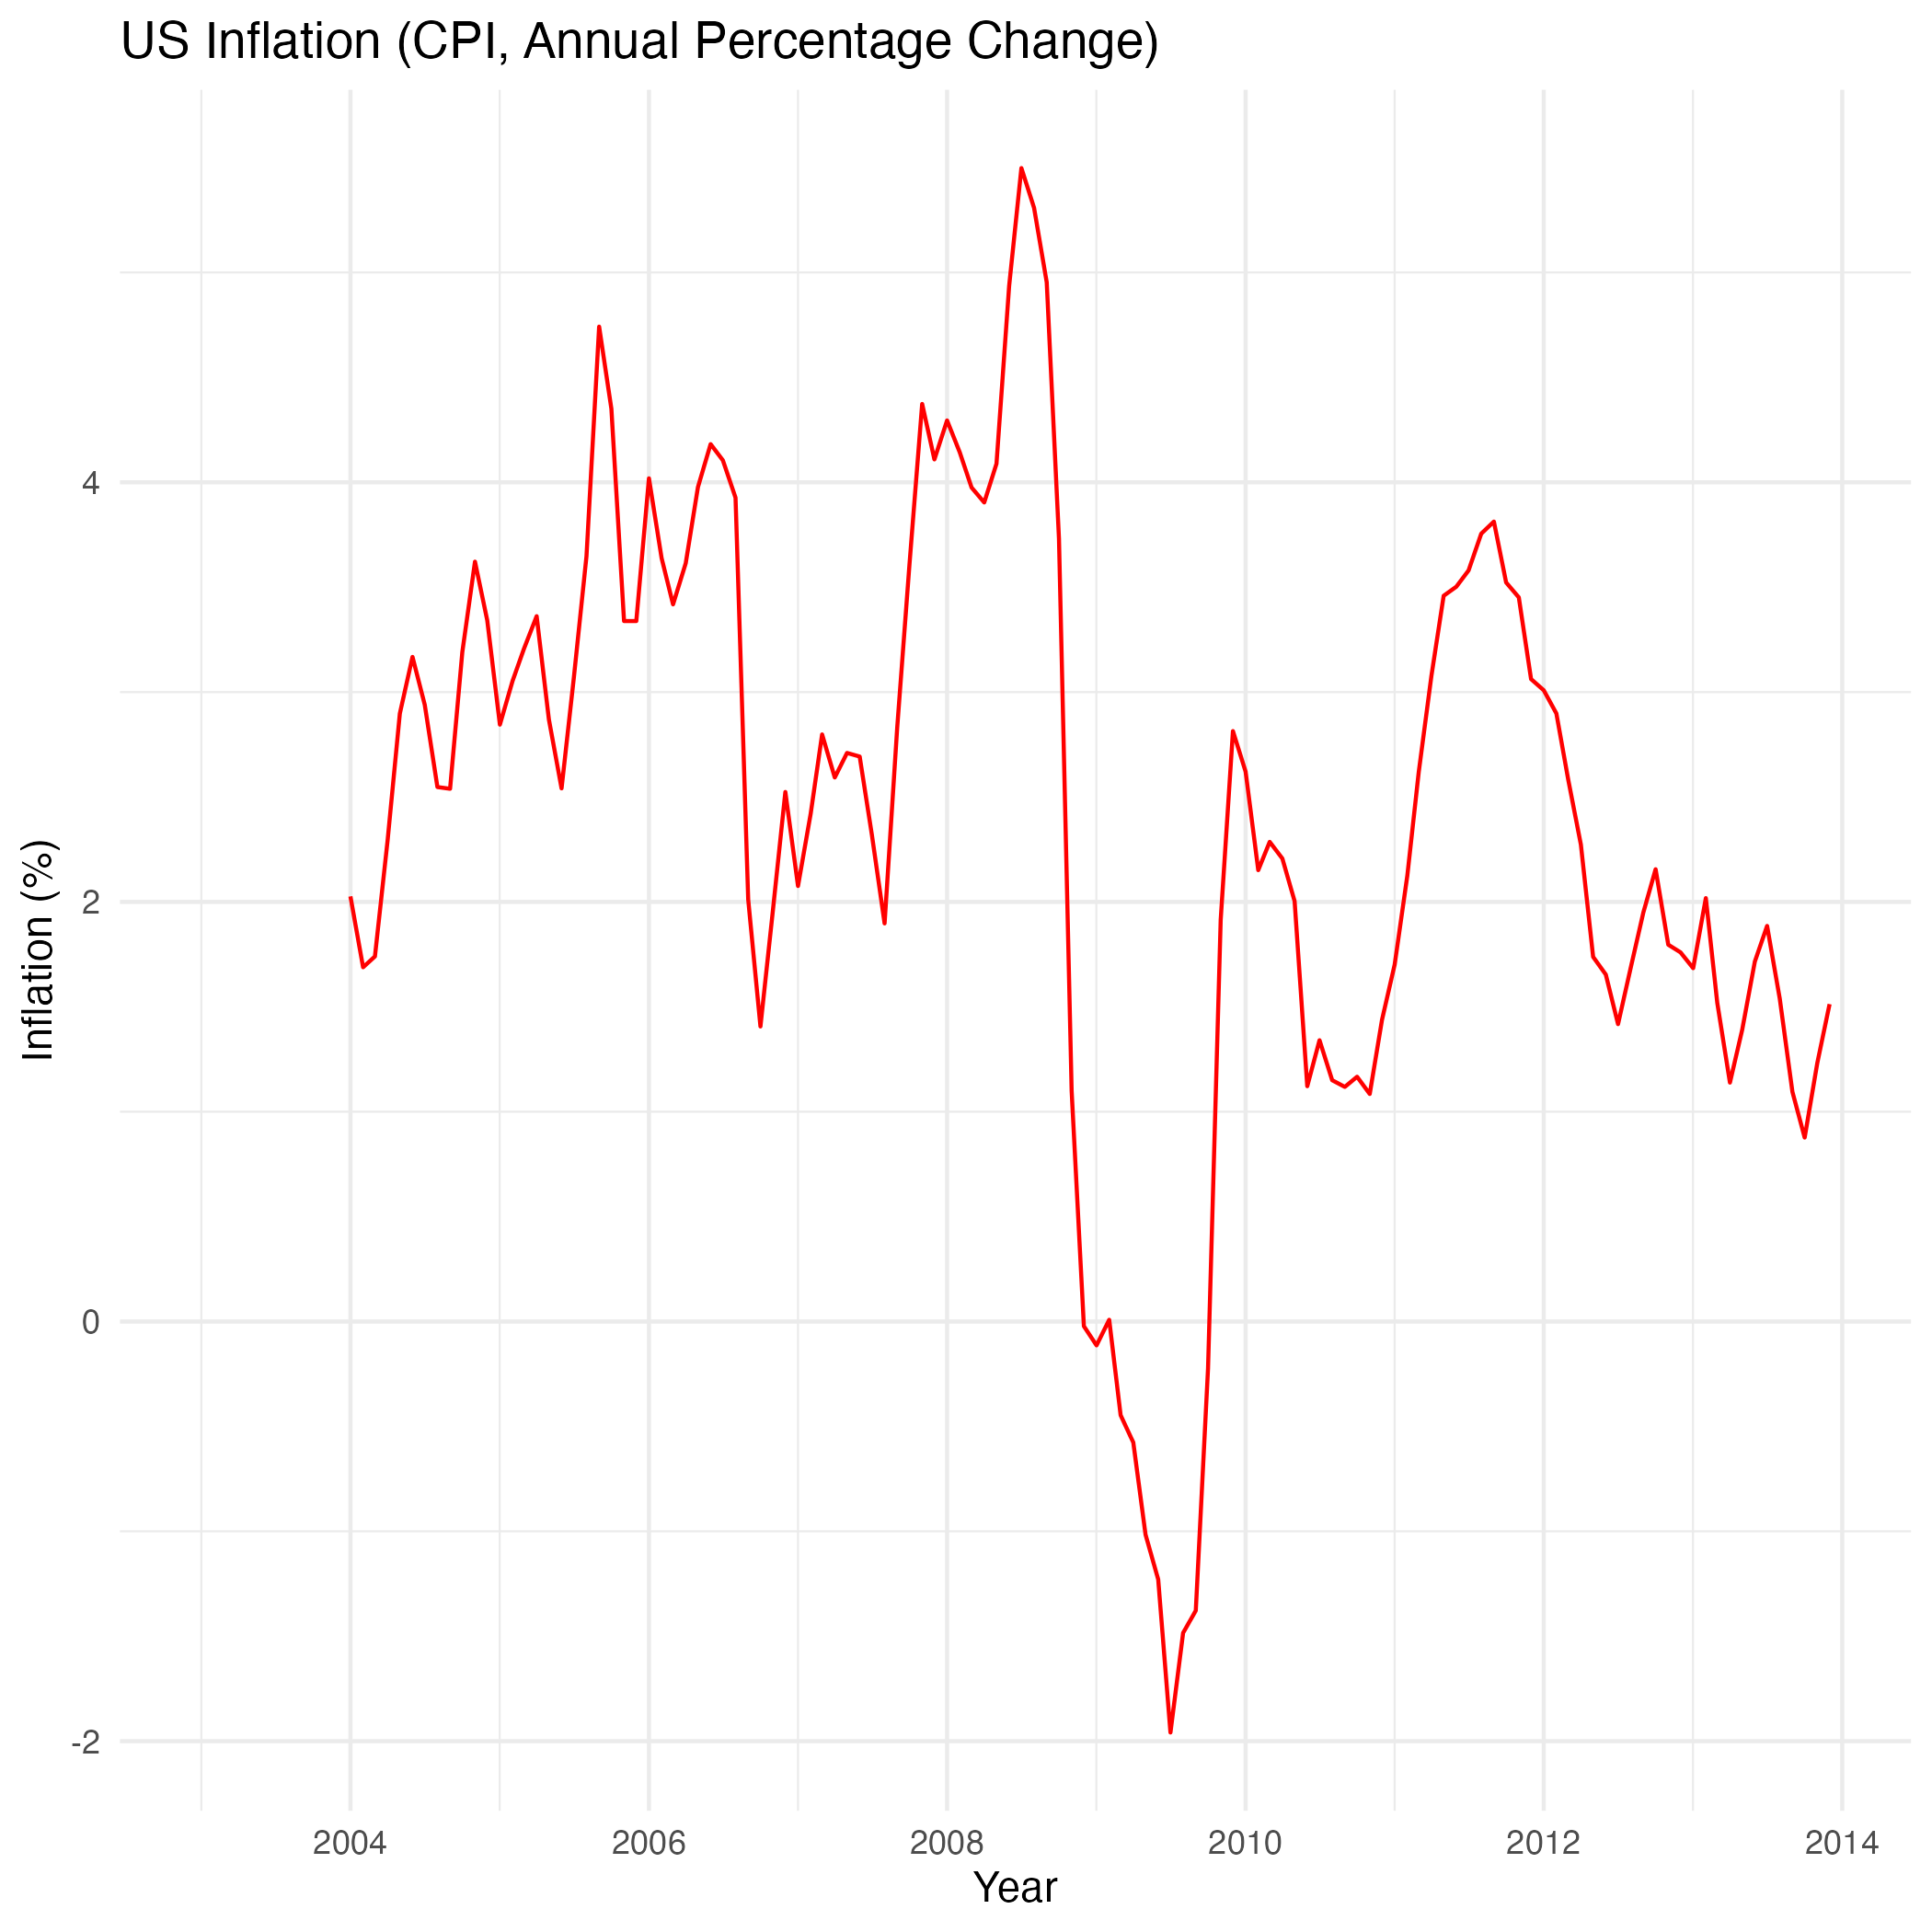
\includegraphics[width=0.8\textwidth]{/Users/cancel/Personal/Coursework/Econ425/FinalWork/R/inflation_graph.png}
    \end{figure}
\end{frame}

\begin{frame}
    \frametitle{Contextual Data --- Interest Rates}
    \begin{itemize}
        \item Tracking the federal funds effective rate from 2003 to 2013.
        \item Significant rate cuts during this period resulted in extended near-zero rates.
        \item Strategy to stimulate the economy by making borrowing cheaper and encouraging spending and investment.
    \end{itemize}
    
\end{frame}
\begin{frame}
    \frametitle{Graph --- Interest Rates}
\begin{figure}[h!]
        \centering
        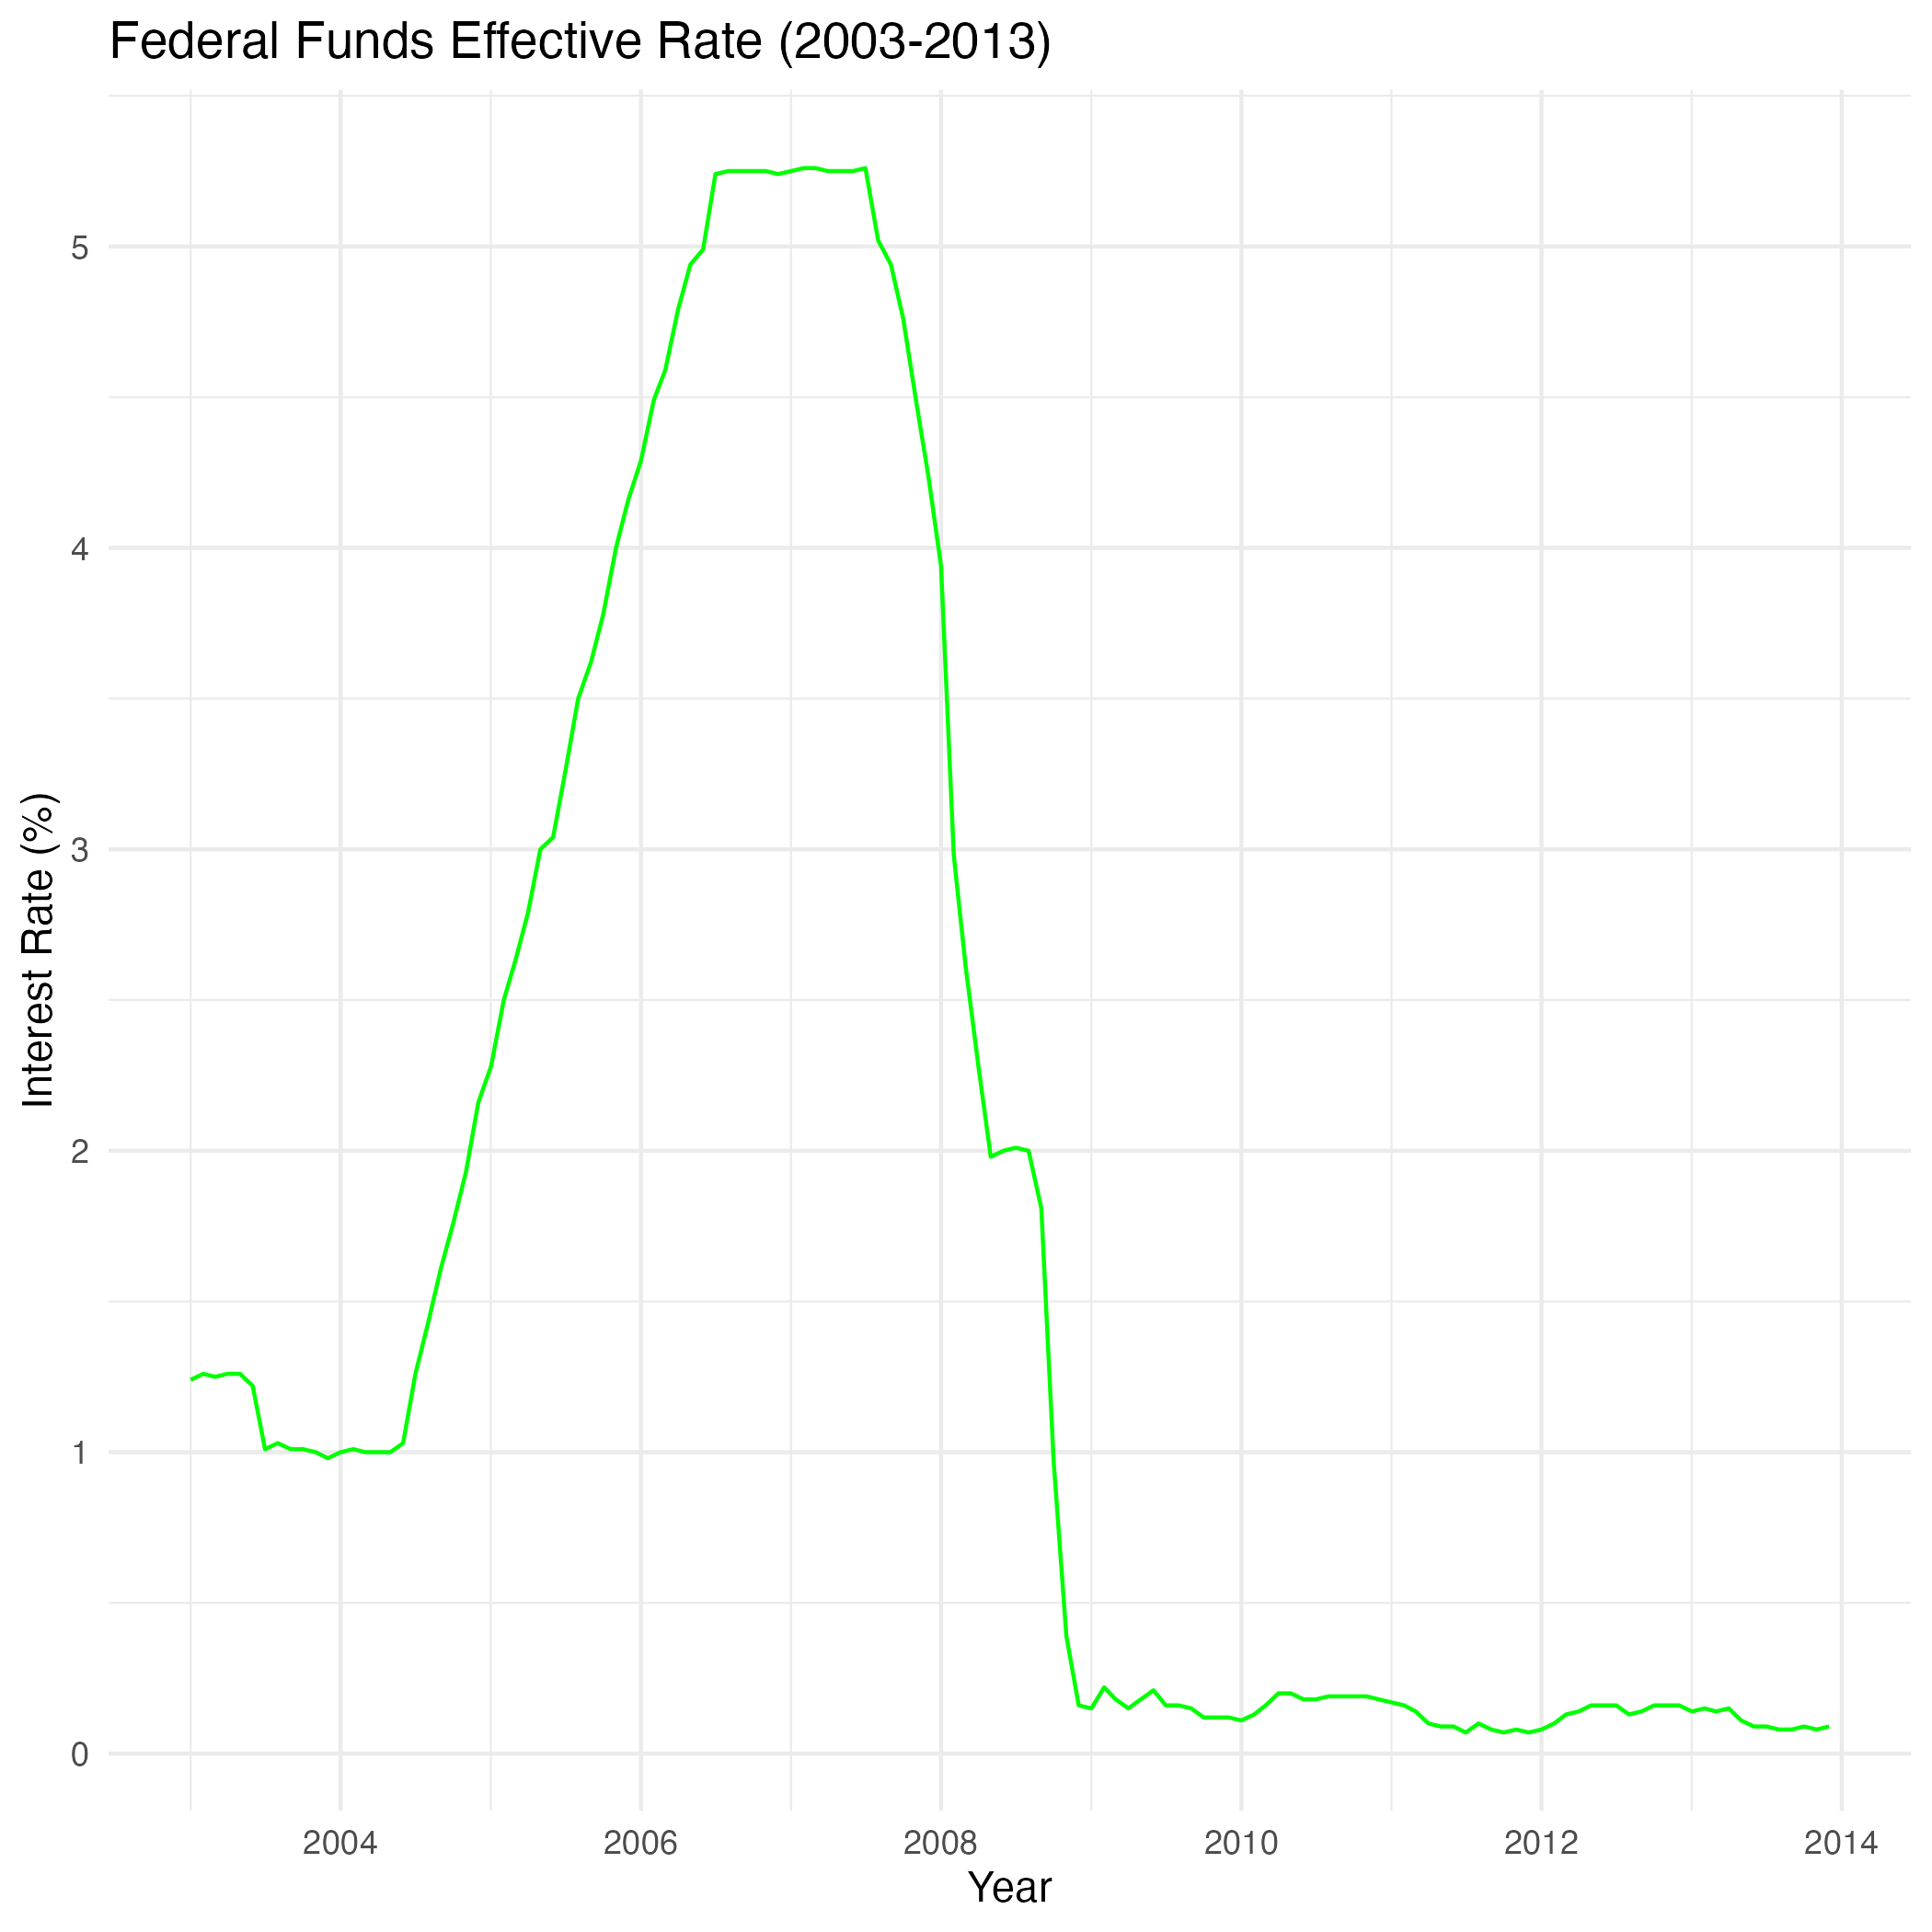
\includegraphics[width=0.8\textwidth]{/Users/cancel/Personal/Coursework/Econ425/FinalWork/R/interest_rate_graph.png}
    \end{figure}
\end{frame}
\begin{frame}
    \frametitle{Contextual Data --- Unemployment Rate}
    \begin{itemize}
        \item Examining the unemployment rate from 2003 to 2013.
        \item Before the recession, the unemployment rate was around a steady 5\%.
        \item Peaked at 10\% in October 2009, indicating the severe impact of the recession on the labor market.
    \end{itemize}

\end{frame}
\begin{frame}
    \frametitle{Graph --- Unemployment Rate}
    \begin{figure}[h!]
        \centering
        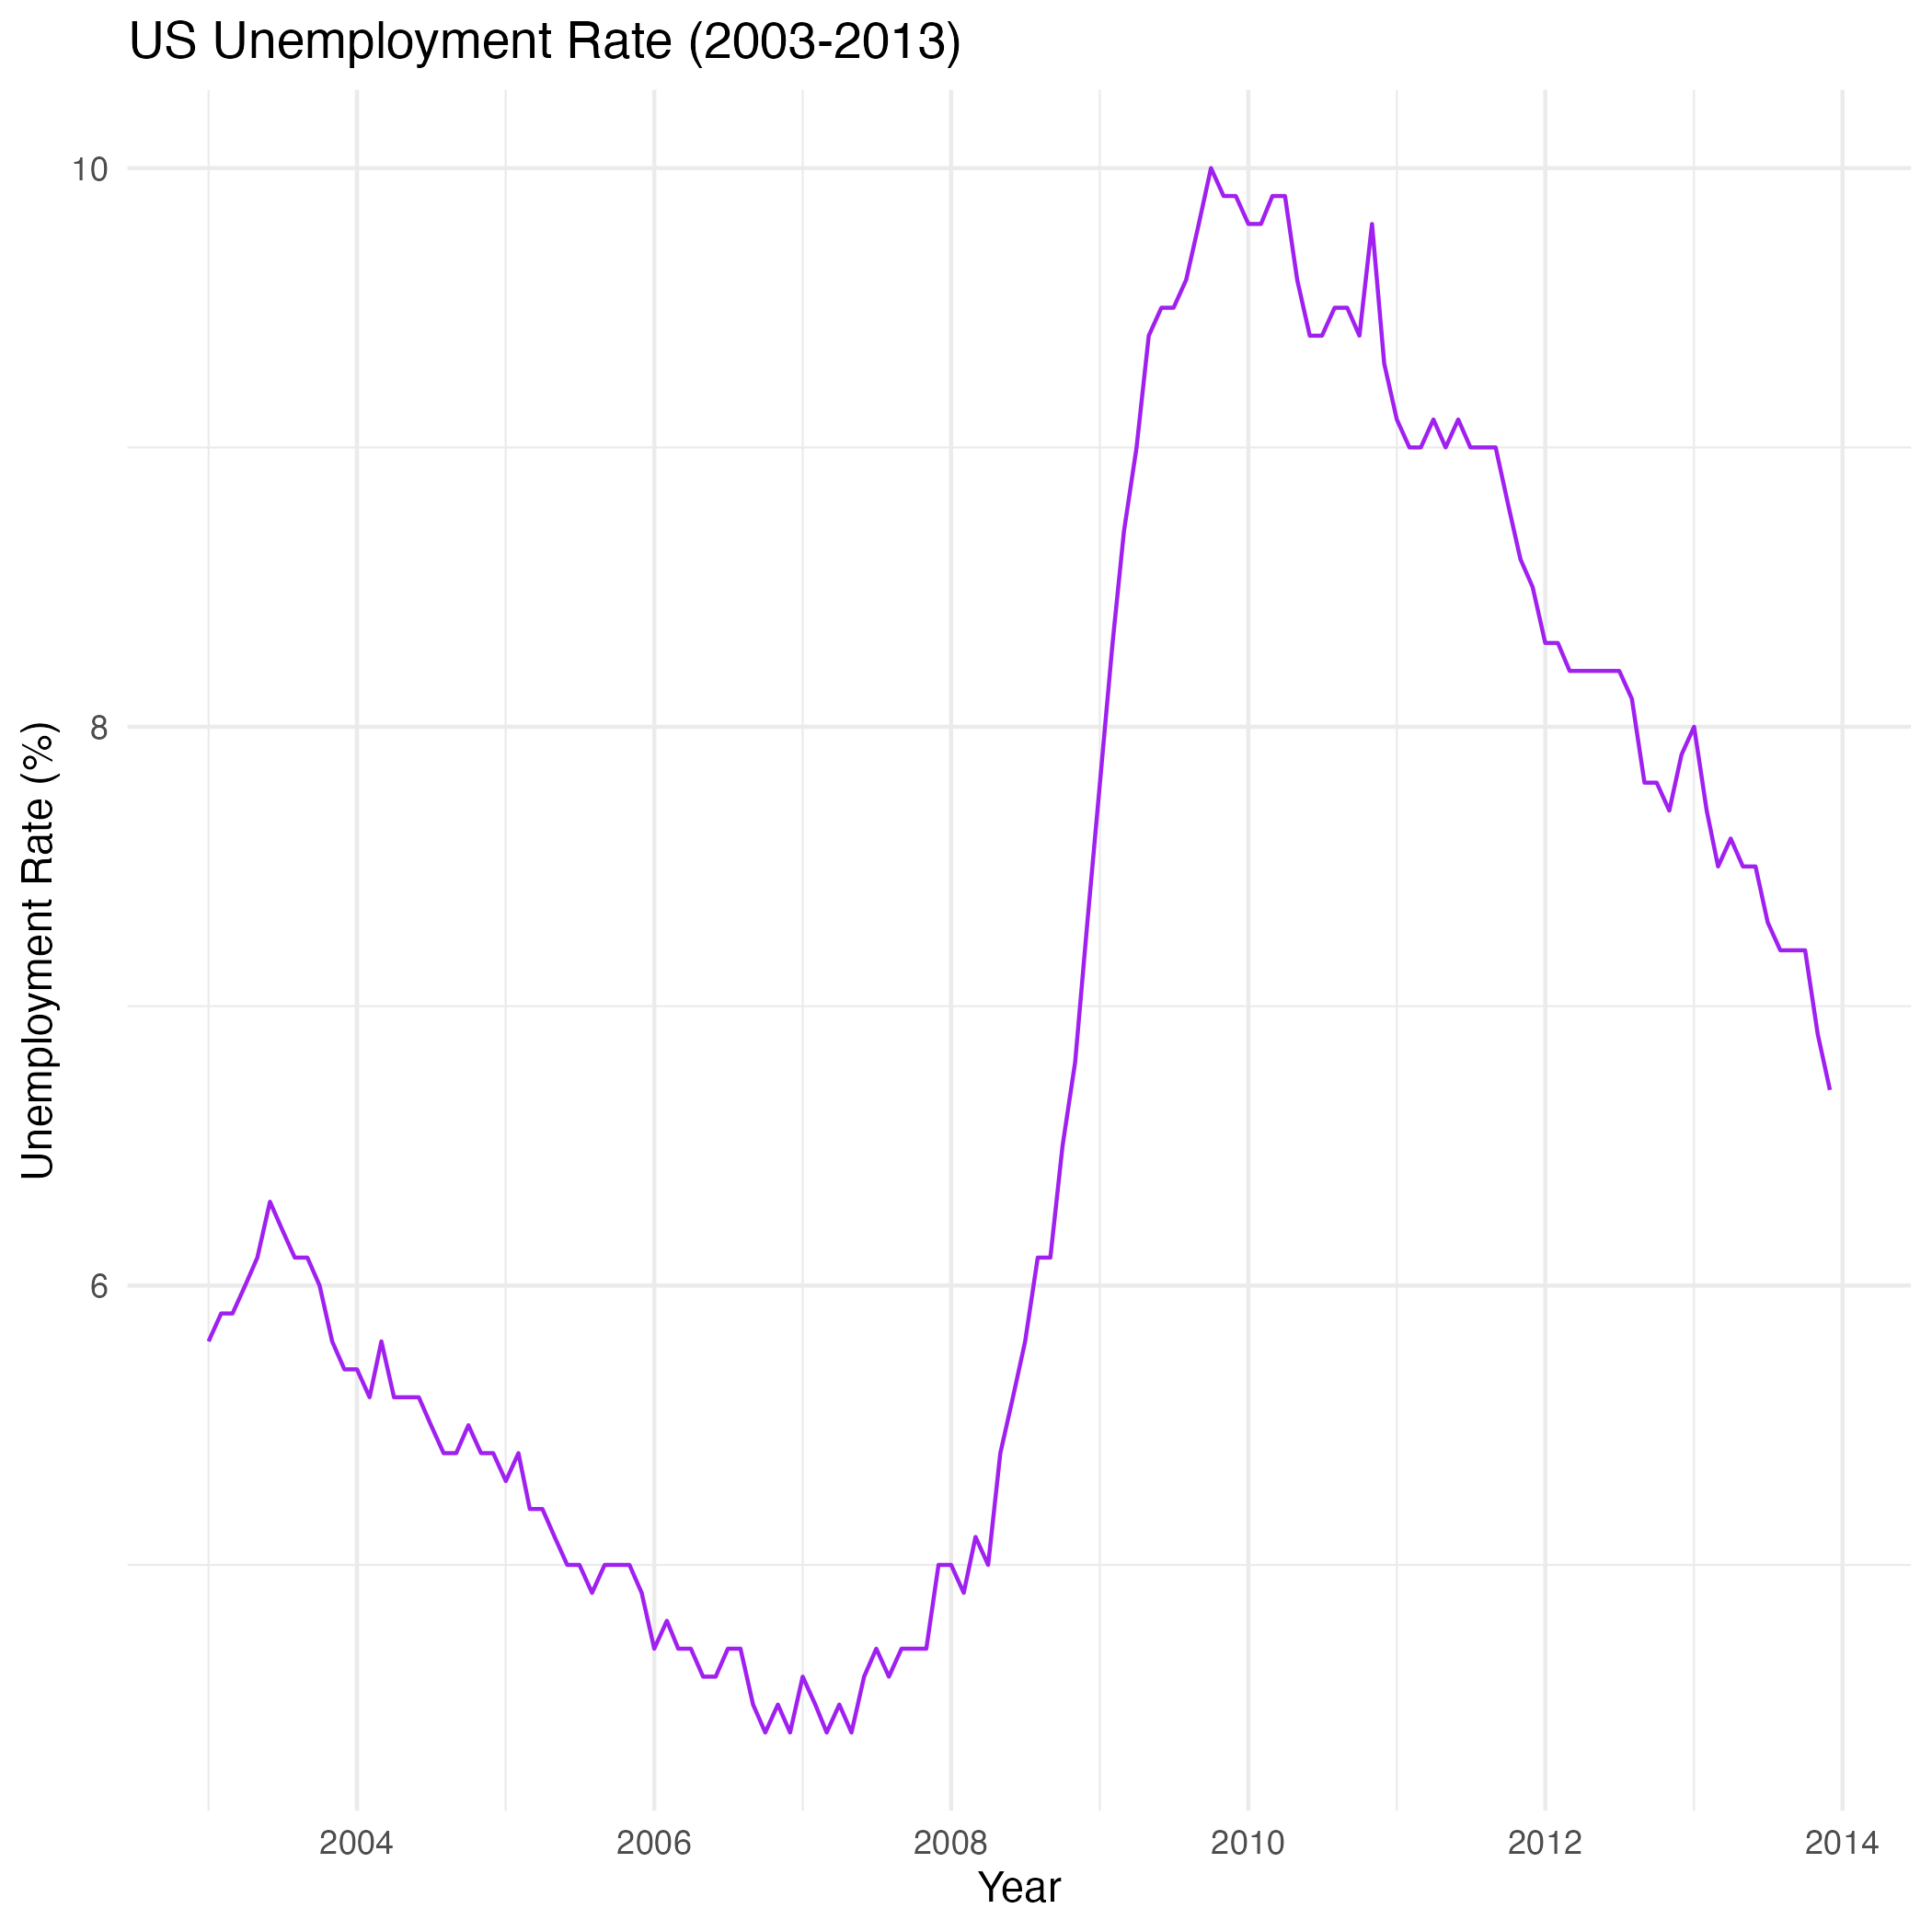
\includegraphics[width=0.8\textwidth]{/Users/cancel/Personal/Coursework/Econ425/FinalWork/R/unemployment_rate_graph.png}
    \end{figure}
\end{frame}
\section{Theory and Decision}
\begin{frame}
    \frametitle{Theory and Decision}
    \begin{itemize}
        \item In the middle of the housing market crisis of 2008 and 2009.
        \item Recommended a monetary policy decision to lower the federal funds rate to around 0.5\% \(\pm \) 0.25\%.
        \item Rationale: Stimulate consumer spending and investment by making borrowing cheaper.
        \item Aim to counteract deflationary pressures and support economic recovery.
        \item Consider implementing a zero interest rate policy and providing effective forward guidance to ensure transparency and manage market expectations.
    \end{itemize}
\end{frame}

\section{Statement}
\begin{frame}
    \frametitle{Statement}
    \textit{The Federal Open Market Committee decided today to lower its target for the federal funds rate by 50 basis points to 0.5 percent. Contributing to this decision has been the continued decline of many economic indicators. In particular, a marked deterioration of labor markets and industrial production have led to a bleak outlook. At the same time, prices have continued to decline, and we now project inflation to be at 1 percent for the next couple of years. In spite of this, the Committee believes that the economy will stabilize in the coming year with the implementation of a new stimulus package. The Fed will continue to closely monitor the economy and reaffirms its promise to ensure economic growth and price stability. If necessary, the Fed is willing to further lower the federal funds rate and maintain a lower interest rate for an extended period to reach this goal.}
\end{frame}

\section{Comparison with Fed's Decision}
\begin{frame}
    \frametitle{Comparison with Fed's Decision}
    \begin{itemize}
        \item The Fed chose to set a target range of 0--0.25\%, which was more aggressive than our recommended target of 0.5\%.
        \item The Fed's decision was likely influenced by the need to provide a stronger immediate boost to the economy during such a critical period.
        \item Additionally, the Fed implemented extra policies to support mortgage and housing markets and facilitate credit extension to households and small businesses.
        \item Given the worsening economic indicators, the Fed's more impactful decision was likely more effective.
    \end{itemize}
\end{frame}

\section{Conclusions}
\begin{frame}
    \frametitle{Conclusions}
    \begin{itemize}
        \item Analysis of the economic conditions in December 2008 highlighted the severity of the recession.
        \item Significant declines in GDP and increases in unemployment.
        \item Recommended monetary policy aimed to stimulate economic activity by lowering interest rates and providing forward guidance.
        \item The Fed's more aggressive approach was likely more effective in providing the necessary economic boost.
        \item Importance of flexibility and responsiveness in monetary policy, particularly during times of economic crisis.
        \item Future policymakers should consider the potential benefits of more aggressive measures when faced with similar challenges.
    \end{itemize}
\end{frame}

\section{Q\&A}
\begin{frame}
    \frametitle{Q\&A}
    Thank you for your attention. This concludes my presentation on the monetary and fiscal policy decisions of December 2008. I hope this has provided a clear understanding of the economic context and the rationale behind policy decisions. If you have any questions, please feel free to ask.
\end{frame}

\end{document}
